\documentclass[]{article}


%-----------------------------------------------------------------------------------------------------------------------------------------
%
%   GLOBALS
%
%-----------------------------------------------------------------------------------------------------------------------------------------
\newcommand{\DOCTITLE}{

}
\newcommand{\DOCAUTHOR}{

}
\newcommand{\DISCLAIMER}
{
    \topskip0pt
    \vspace*{\fill}
    {
    \centering
        \small{
            THIS DOCUMENT IS INTENDED FOR CANADIAN TEAMS ONLY
        }
    }
    \\
    {
    \centering
        \small{
        GO CANADA 
        }
    }
    \vspace*{\fill}
}

\usepackage{lmodern}
\usepackage{amssymb,amsmath}
\usepackage{ifxetex,ifluatex}
\usepackage{fixltx2e} % provides \textsubscript
\ifnum 0\ifxetex 1\fi\ifluatex 1\fi=0 % if pdftex
  \usepackage[T1]{fontenc}
  \usepackage[utf8]{inputenc}
\else % if luatex or xelatex
  \ifxetex
    \usepackage{mathspec}
    \usepackage{xltxtra,xunicode}
  \else
    \usepackage{fontspec}
  \fi
  \defaultfontfeatures{Mapping=tex-text,Scale=MatchLowercase}
  \newcommand{\euro}{€}
\fi
% use upquote if available, for straight quotes in verbatim environments
\IfFileExists{upquote.sty}{\usepackage{upquote}}{}
% use microtype if available
\IfFileExists{microtype.sty}{%
\usepackage{microtype}
\UseMicrotypeSet[protrusion]{basicmath} % disable protrusion for tt fonts
}{}
\ifxetex
  \usepackage[setpagesize=false, % page size defined by xetex
              unicode=false, % unicode breaks when used with xetex
              xetex]{hyperref}
\else
  \usepackage[unicode=true]{hyperref}
\fi
\usepackage[usenames,dvipsnames]{color}
\hypersetup{breaklinks=true,
            bookmarks=true,
            pdfauthor={},
            pdftitle={Canadian Amateur Rocketry Standards and Best Practices},
            colorlinks=true,
            citecolor=blue,
            urlcolor=blue,
            linkcolor=magenta,
            pdfborder={0 0 0}}
\urlstyle{same}  % don't use monospace font for urls
\usepackage{longtable,booktabs}
\usepackage{graphicx,grffile}
\makeatletter
\def\maxwidth{\ifdim\Gin@nat@width>\linewidth\linewidth\else\Gin@nat@width\fi}
\def\maxheight{\ifdim\Gin@nat@height>\textheight\textheight\else\Gin@nat@height\fi}
\makeatother
% Scale images if necessary, so that they will not overflow the page
% margins by default, and it is still possible to overwrite the defaults
% using explicit options in \includegraphics[width, height, ...]{}
\setkeys{Gin}{width=\maxwidth,height=\maxheight,keepaspectratio}
\usepackage[normalem]{ulem}
% avoid problems with \sout in headers with hyperref:
\pdfstringdefDisableCommands{\renewcommand{\sout}{}}
\setlength{\parindent}{0pt}
\setlength{\parskip}{6pt plus 2pt minus 1pt}
\setlength{\emergencystretch}{3em}  % prevent overfull lines
\providecommand{\tightlist}{%
  \setlength{\itemsep}{0pt}\setlength{\parskip}{0pt}}
\setcounter{secnumdepth}{0}

\title{Canadian Amateur Rocketry Standards and Best Practices}
\date{}

% Redefines (sub)paragraphs to behave more like sections
\ifx\paragraph\undefined\else
\let\oldparagraph\paragraph
\renewcommand{\paragraph}[1]{\oldparagraph{#1}\mbox{}}
\fi
\ifx\subparagraph\undefined\else
\let\oldsubparagraph\subparagraph
\renewcommand{\subparagraph}[1]{\oldsubparagraph{#1}\mbox{}}
\fi

%-----------------------------------------------------------------------------------------------------------------------------------------
%
%   PAGE SIZE AND MARGINS
%
%-----------------------------------------------------------------------------------------------------------------------------------------
\usepackage[a4paper,headheight=30pt]{geometry}
%\usepackage[letterpaper, portrait, margin=2in]{geometry}
\addtolength{\topmargin}{-.5in}
\addtolength{\textheight}{1.75in}

\usepackage{graphicx}

\usepackage{fancyhdr}
\pagestyle{fancy}


%-----------------------------------------------------------------------------------------------------------------------------------------
% Page break after sections
%-----------------------------------------------------------------------------------------------------------------------------------------
%\usepackage{titlesec}
%\newcommand{\sectionbreak}{\clearpage}

\lhead{
    %left header content
%    \topskip0pt
%    \vspace*{\fill}
    {
    \centering
        
\includegraphics[height=2.66em]{images/mapleleaf.png}
    }
%    \vspace*{\fill}
}
\chead{
    \topskip0pt
    \vspace*{\fill}
    {
    \centering
        \small{
            THIS DOCUMENT IS INTENDED FOR CANADIAN TEAMS ONLY
        }
    }
    \\
    {
    \centering
        \small{
        GO CANADA 
        }
    }
    \vspace*{\fill}
}
\rhead{
%    \topskip0pt
%    \vspace*{\fill}
    % right header content
    {
    \centering
        
\includegraphics[height=3.0em]{images/mapleleaf.png}
    }
%    \vspace*{\fill}
}
\lfoot{
    % left footer content
    \topskip0pt
    \vspace*{\fill}
    Canada
    Revision 0.0
    \vspace*{\fill}
}
\cfoot{
    % middle footer content
    \topskip0pt
    \vspace*{\fill}
    {
    \centering
    Doc Template \\
    \today
    }
    \vspace*{\fill}
}
\rfoot{
    % right footer content
    \topskip0pt
    \vspace*{\fill}
    \thepage
    \vspace*{\fill}
}
% extend the header into the margins
\usepackage{calc}
\fancyheadoffset[L,R]{\marginparsep+\marginparwidth}

%--------------------------------------------------------------------------------------------------------------
%	My Packages
%--------------------------------------------------------------------------------------------------------------
\usepackage{capt-of}
%--------------------------------------------------------------------------------------------------------------
%	
%	COPY FRONTMATTER AND MAINMATTER AND BACKMATTER COMMANDS
%	
%--------------------------------------------------------------------------------------------------------------
\makeatletter

\newcommand\frontmatter{%
    \cleardoublepage
  %\@mainmatterfalse
  \pagenumbering{roman}}

\newcommand\mainmatter{%
    \cleardoublepage
 % \@mainmattertrue
  \pagenumbering{arabic}}

\newcommand\backmatter{%
  \if@openright
    \cleardoublepage
  \else
    \clearpage
  \fi
 % \@mainmatterfalse
   }

\makeatother

%--------------------------------------------------------------------------------------------------------------
%
%	BEGIN DOCUMENT
%
%--------------------------------------------------------------------------------------------------------------
\begin{document}

%--------------------------------------------------------------------------------------------------------------
%
%	TITLEPAGE
%
%--------------------------------------------------------------------------------------------------------------

%\maketitle

\begin{titlepage}

\newcommand{\HRule}{\rule{\linewidth}{0.5mm}} % Defines a new command for the horizontal lines, change thickness here

\center % Center everything on the page
 
%----------------------------------------------------------------------------------------
%	HEADING SECTIONS
%----------------------------------------------------------------------------------------


\includegraphics[width=200pt]{images/mapleleaf.png}\\[1cm] % Include a logo - this will require the graphicx package
\textsc{\Large Reaction Dynamics Inc.}\\[0.5cm] % Major heading such as course name
\textsc{\large Operations Division}\\[0.5cm] % Minor heading such as course title

%----------------------------------------------------------------------------------------
%	LOGO SECTION
%----------------------------------------------------------------------------------------

\begin{figure}[ht]
    \centering
    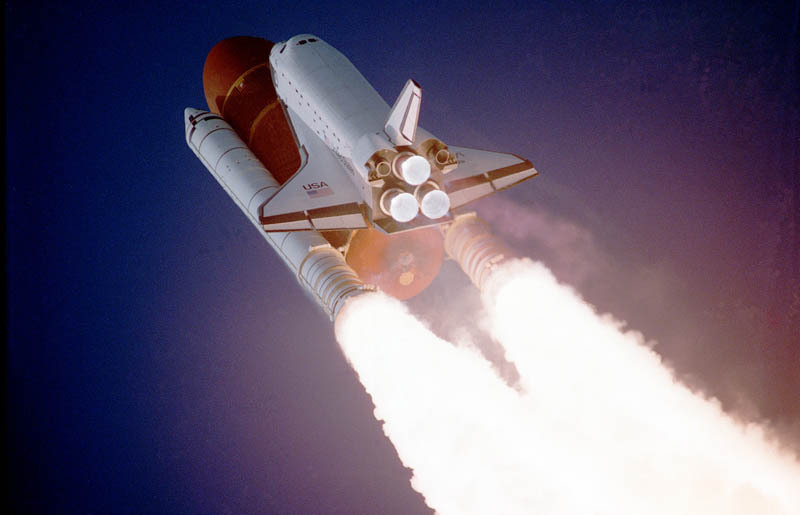
\includegraphics[height=200pt]{images/nasa-rocket-launch-high-quality-24.jpg}\\
\end{figure}

%----------------------------------------------------------------------------------------
%	TITLE SECTION
%----------------------------------------------------------------------------------------

\HRule \\[0.6cm]
{ \Huge \bfseries 
SLV Operations Outline and Field Schedule
}\\[0.4cm] 

\HRule \\[1cm]
 
%----------------------------------------------------------------------------------------
%	AUTHOR SECTION
%----------------------------------------------------------------------------------------
\begin{minipage}{0.4\textwidth}
\begin{flushleft} \large
	\begin{tabular} {r l} 
        \emph{Author(s):} & Someone	\\
	\end{tabular}
\end{flushleft}
\end{minipage}
~
\begin{minipage}{0.4\textwidth}
\begin{flushright} \large
	\begin{tabular} {r l} 
		\emph{Coordinator:} & Someone 		\\
		\emph{Supervisor:}  & Someone 		\\
		\emph{EIR:}         & Someone  		        \\
	\end{tabular}
\end{flushright}
\end{minipage}\\[2cm]

%----------------------------------------------------------------------------------------
%	DATE SECTION
%----------------------------------------------------------------------------------------

{\large \today}\\[2cm] % Date, change the \today to a set date if you want to be precise

\vfill % Fill the rest of the page with whitespace

\end{titlepage}


%--------------------------------------------------------------------------------------------------------------
%
%	FRONT MATTER
%
%--------------------------------------------------------------------------------------------------------------
\frontmatter
%\section*{Abstract}
\begin{abstract}
The following document is a compiled set of standards and best practices that the Canadian Teams have agreed to abide by and contribute to. The goal of the document is to provide standards which ensure the safe operations of the Canadian rocketry teams, and the successful operation of their rockets, so that they may remain competitive at whatever international competition they choose to participate in (in the case of this document, the chosen competition is the Spaceport America Cup). The document will also provide the best practices for designing, analyzing, manufacturing and testing a rocket to provide the best possible performance in competition. The document will be maintained and updated by the Canadian teams, who will make sure the methods presented herein are the most recent and effective, and that new methods and mechanisms are documented for the use of other Canadian teams.
\end{abstract}
\clearpage

{
\hypersetup{linkcolor=black}
\setcounter{tocdepth}{3}
\tableofcontents
\clearpage
}

\listoftables
\listoffigures
\clearpage


%--------------------------------------------------------------------------------------------------------------
%
%	MAIN MATTER
%
%--------------------------------------------------------------------------------------------------------------
\mainmatter

%--------------------------------------------------------------------------------------------------------------
% body
%--------------------------------------------------------------------------------------------------------------
\subsection{List of Abbreviations}\label{list-of-abbreviations}
\begin{longtable}[c]{@{}llll@{}}
\toprule
Abbreviation & Description & Function of & Units\tabularnewline
\midrule
\endhead
AOA, \(\alpha\) & Angle of Attack & & radians\tabularnewline
COP & Center of pressure & & N/A\tabularnewline
COG & Center of gravity & time & N/A\tabularnewline
Re & Reynolds Number & \( \rho,\mu,\vec{v},L \) &
dimensionless\tabularnewline
\(Re_{crit}\) & Critical Reynolds Number & \( \rho,\mu,\vec{v},L \) &
dimensionless\tabularnewline
\(I_{zz}\) & Pitch/Yaw Moment of Inertia & time & \(m^4\)\tabularnewline
D & Drag Force (combined) & & N\tabularnewline
W & Weight of the Rocket & & N\tabularnewline
R & Specific Gas Constant & & \(J kg^{-1} K^{-1}\)\tabularnewline
T & Thrust of the Rocket & & N\tabularnewline
\(t_f\) & Fin thickness & distance & m\tabularnewline
\(L_{cf}\) & Aerodynamic Chord Length of Fins & distance &
m\tabularnewline
c & Speed of sound & \( \sqrt{\gamma RT} \) &\tabularnewline
\(R_a\) & Surface Finish & \( distance \) & microns\tabularnewline
M & Mach Number & \( \vec{v}, c \) & dimensionless\tabularnewline
\(D_{pa}, C_{pa}\) & Parasitic Drag Force, Coefficient &
&\tabularnewline
\(D_{fb}, C_{fb}\) & Body Drag Force, Coefficient & &\tabularnewline
\(D_{fp}, C_{fp}\) & Fin Pressure Drag Force, Coefficient &
&\tabularnewline
\(D_{pr}, C_{pr}\) & Pressure Drag Force, Coefficient & &\tabularnewline
\(D_{in}, C_{in}\) & Interference Drag Force, Coefficient &
&\tabularnewline
\(D_{ba}, C_{ba}\) & Base Drag Force, Coefficient & &\tabularnewline
\(D_{sk}, C_{sk}\) & Skin Friction Drag Force, Coefficient &
&\tabularnewline
\(D_{aoa}, C_{aoa}\) & Additional Angle of Attack Drag Force,
Coefficient & &\tabularnewline
\(C_{MC}\) & Corrective Moment Coefficient & &\tabularnewline
\(C_{FN}\) & Normal Force Coefficient & &\tabularnewline
\(C_{PDM}\) & Propulsive Damping Moment Coefficient & &\tabularnewline
\(C_{ADM}\) & Aerodynamic Damping Moment Coefficient & &\tabularnewline
\(A_{wb}\) & Area of Wetted Body & & \(m^2\)\tabularnewline
\(A_{wf}\) & Area of Wetted Fins & & \(m^2\)\tabularnewline
\(A_{fr}\) & Frontal Reference Area & & \(m^2\)\tabularnewline
\(A_{fp}\) & Fin Planform Area & & \(m^2\)\tabularnewline
\(A_{fe}\) & Exposed Fin Planform Area & & \(m^2\)\tabularnewline
OD,\(\phi_{bt}\) & Outer Diameter & & m\tabularnewline
L & Total Length of Rocket & & m\tabularnewline
h\_n & Height of the nose cone & & m\tabularnewline
\(S_{fc}\) & Thrust Specific Fuel Consumption & &
\(\dfrac{g}{s}\cdot \dfrac{1}{N} = \dfrac{s}{m}\)\tabularnewline
\(\dot{m}_{fc}\) & Mass Flow Rate due to Fuel Consumption & &
\(\dfrac{g}{s}\cdot \dfrac{1}{N} = \dfrac{s}{m}\)\tabularnewline
\(T_{avg}\) & Average Thrust & & N\tabularnewline
\(t_{burn}\) & Burn Time & & s\tabularnewline
\(m_{m_t}\) & Total Motor Mass & & g\tabularnewline
\(W_{m_t}\) & Total Motor Weight & & N\tabularnewline
\(F_N\) & Aerodynamic Normal Force & & N\tabularnewline
\(F_A\) & Aerodynamic Axial Force & & N\tabularnewline
\(F_L\) & Aerodynamic Lift Force & & N\tabularnewline
\(S_{lm}\) & Longitudinal Stability Margin & & Calibers\tabularnewline
\(f_B\) & Fineness Ratio & & dimensionless\tabularnewline
\(\mu\) & Dynamic Viscosity & & \(N s / m^2\)\tabularnewline
\(\nu\) & Kinematic Viscosity & \(\mu\), \(\rho\) &
\(m^2/s\)\tabularnewline
\(\lambda\) & Angular Acceleration & & \(rad/s^2\)\tabularnewline
\(\omega\) & Angular Velocity & & \(rad/s\)\tabularnewline
\(\theta\) & Angular Position & & \(radians\)\tabularnewline
\bottomrule
\end{longtable}

\captionof{table}{List of Abbreviations}
\clearpage

\section{Section 0 - Explanation of the Standards}\label{section-0}
	% section 1

\subsection{Section 1}\label{section1}

some text goes here


	\clearpage

\section{Section 1 - Flight Dynamics, Prediction and Simulation}\label{section-1}
	% section 1

\subsection{Section 1}\label{section1}

some text goes here


	\clearpage
	
\section{Section 2 - Aerostructures}\label{section-2}
	% section 1

\subsection{Section 1}\label{section1}

some text goes here


	\clearpage
	
\section{Section 3 - Recovery Systems}\label{section-3}
	% section 1

\subsection{Section 1}\label{section1}

some text goes here


	\clearpage
	
\section{Section 4 - Payloads}\label{section-0}
	% section 1

\subsection{Section 1}\label{section1}

some text goes here


	\clearpage
	
\section{Section 5 - Avionics and Groundstations}\label{section-4}
	% section 1

\subsection{Section 1}\label{section1}

some text goes here


	\clearpage
	
\section{Section 6 - Propulsion}\label{section-5}
	% section 1

\subsection{Section 1}\label{section1}

some text goes here


	\clearpage
	
\section{Section 7 - Competition and Field Operations}\label{section-6}
	% section 1

\subsection{Section 1}\label{section1}

some text goes here


	\clearpage
	
\section{Section 8 - General Testing and Documentation Guidelines}\label{section-7}
	% section 1

\subsection{Section 1}\label{section1}

some text goes here


	\clearpage
	
\section{Section 9 - Policy of the Standards}\label{section-8}
	% section 1

\subsection{Section 1}\label{section1}

some text goes here


	\clearpage

%--------------------------------------------------------------------------------------------------------------
%
%	BACK MATTER
%
%--------------------------------------------------------------------------------------------------------------
%\backmatter

%--------------------------------------------------------------------------------------------------------------
%--------------------------------------------------------------------------------------------------------------
\mainmatter
\end{document}
